\documentclass[a4paper,usenatbib]{aspdoc}
\usepackage{newtxtext,newtxmath}
\usepackage{ae,aecompl}
\usepackage{graphicx}	% Including figure files
\usepackage{amsmath}	% Advanced maths commands
\usepackage{amssymb}	% Extra maths symbols
\usepackage{lipsum}
\usepackage{float}
\usepackage{multirow}
\usepackage{booktabs}
\usepackage{geometry}
\usepackage[load=prefixed]{siunitx}
\sisetup{output-decimal-marker = {,}}
\geometry{left=25mm,right=25mm,top=25mm,bottom=25mm}

\usepackage[numbers]{natbib}
\setcitestyle{numbers}

\newcounter{simplecount}
\setcounter{simplecount}{0}
\renewcommand{\theequation}{\arabic{simplecount}}
\newcommand{\owncount}{\refstepcounter{simplecount}}

% Title
\title[]{BRU: Brückenschaltung}

% The list of authors
\author[]{
    Riedel Lisa, Wegmann Peter
    \newauthor
    \,Gruppe 6
}

% Don't change these lines
\begin{document}
    \label{firstpage}
    \pagerange{\pageref{firstpage}--\pageref{lastpage}}
    \maketitle
    
    

    % Body
    \section{Einleitung}\label{sec:intro}
       Dieser Versuch kann im Allgemeinen in zwei Teile unterteilt werden. Im ersten Teil wird mittels Wheatstonescher Brückenschaltung Widerstände von verschiedenen elektronischen Bauteilen gemessen. Unter anderem werden die Widerstände von verschiedenen Spulen, eines Potentiometers und einer Glühlampe bestimmt.\\
       Im zweiten Teil werden, mittels Wechselspannungsbrücke, Induktivitäten von Spulen und die Kapazität eines Kondensators gemessen.
                
    
    \section{Verwendete Methoden}\label{sec:method}
        \subsection{Wheatstonesche Brücke}\label{subsec:method_wheatstone}
            Hierbei handelt es sich um eine elektronische Schaltung wie in Abbildung \ref{fig:kreis} aufgeführt.
            Für die korrekte Versuchsdurchführung muss lediglich die oben genannte Schaltung aufgebaut werden. Anschließend können die Messungen unternommen und aufgezeichnet werden. Hierbei verwendet man nach Abgleichen der Schaltung, Formel \ref{eq:wheatstone_abgleich} zur Berechnung der Widerstände. Um die Schaltung abzugleichen, wird das Potentiometer so lange verändert, bis das Nullinstrument keinen Ausschlag mehr anzeigt. 
            \begin{equation}
                \owncount
                \frac{R_1}{R_2} = \frac{R_3}{R_4} = \frac{A}{10 - A}
                \label{eq:wheatstone_abgleich}
            \end{equation}
            Bei $A$ handelt es sich um die Anzahl der Umdrehungen am Zehngangpotentiometer. $R_1$ bis $R_4$ sind die verwendeten Widerstände.
        
        \subsection{Wechselspannungsbrücke}\label{subsec:method_wechsel}
            Auch hierbei handelt es sich um eine elektronische Schaltung wie in Abbildung 5 der Anleitung \cite{anleitung} aufgeführt. Diese Schaltung ist besonders nützlich um Kapazitäten und Induktivitäten mittels Abgleichbedingung \ref{eq:abgleich2} und Bestimmungsgleichung \ref{eq:bestimmung} zu bestimmen.
            \\
            Um mit den Messungen der Bauteile zu beginnen wird die oben genannte Schaltung aufgebaut. Man beachte hierbei, dass mittels Funktionsgenerator eine Wechselspannung $U(t)$ mit kleiner Amplitude ($\leq 2,0 \mathrm{V}$) angelegt wird. Dieser dient anschließend, zusammen mit der Spannung $U_g (t)$ zwischen Punkten b und d \cite{anleitung}, der Visualisierung des Phasenverschiebung beider Spannungen. Mit Hilfe der Darstellung der Lissajous-Figur können die Phasenwinkel $\Psi_1, \Psi_2$ von $U(t)$ und $U_g (t)$ gleichgesetzt werden. Damit lassen sich die gesuchten Induktivitäten und Kapazitäten über die vereinfachte Gleichung \ref{eq:wechsel_abgleich} berechnen. Dies ist möglich, da $\Psi_1 = \Psi_2$ nach dem Abgleichvorgang. Somit können die $\cot(\Psi_1), \cot(\Psi_1)$ Terme aus Gleichung 17 der Anleitung \cite{anleitung} gekürzt werden.
            \begin{equation}
                \owncount
                \frac{Z_1}{Z_2} = \frac{A}{10 - A}
                \label{eq:wechsel_abgleich}
            \end{equation}
            Bei $Z_1$ und $Z_2$ handelt es sich um komplexe Widerstände. Für unterschiedliche Bauteile werden hierbei unterschiedliche Werte gewählt.
            \\
            Man beachte die Verwendung der in der Anleitung angeführten Reaktanzbrücke. Diese ist in Abbildung 5 der Anleitung \cite{anleitung} durch ein liegendes Dreieck dargestellt. Dabei handelt es sich um ein elektronisches Bauteil, welches zur Darstellung der Lissajous-Figuren verwendet wird. Würde diese nicht verwendet werden, so könnte das Oszilloskop $U_g(t)$ zu $U(t)$ nicht visualisieren, da das direkte Abgreifen von $U_g(t)$ einem kurzschließen einer Masche gleichkommt. Zudem verwendet man für das Abgleichen der Brücke eine Vergleichsspule $L_v$, sowie Vergleichskondensator $C_v$. $L_v$ wird bei Messung von $L_x$ verwendet, $C_v$ bei der Messung von $C_x$.\\
            Für die Berechnung der verbrauchten Leistung $P_x$ an der Lampe, wird Formel \ref{eq:leist} verwendet.
            \begin{equation}
            \owncount
                P = R_x \cdot I^2 
                \label{eq:leist}
            \end{equation}
            Hier bezeichnet $U$ die Spannung und $I$ den Strom.  
        
            \begin{figure}
                \centering
                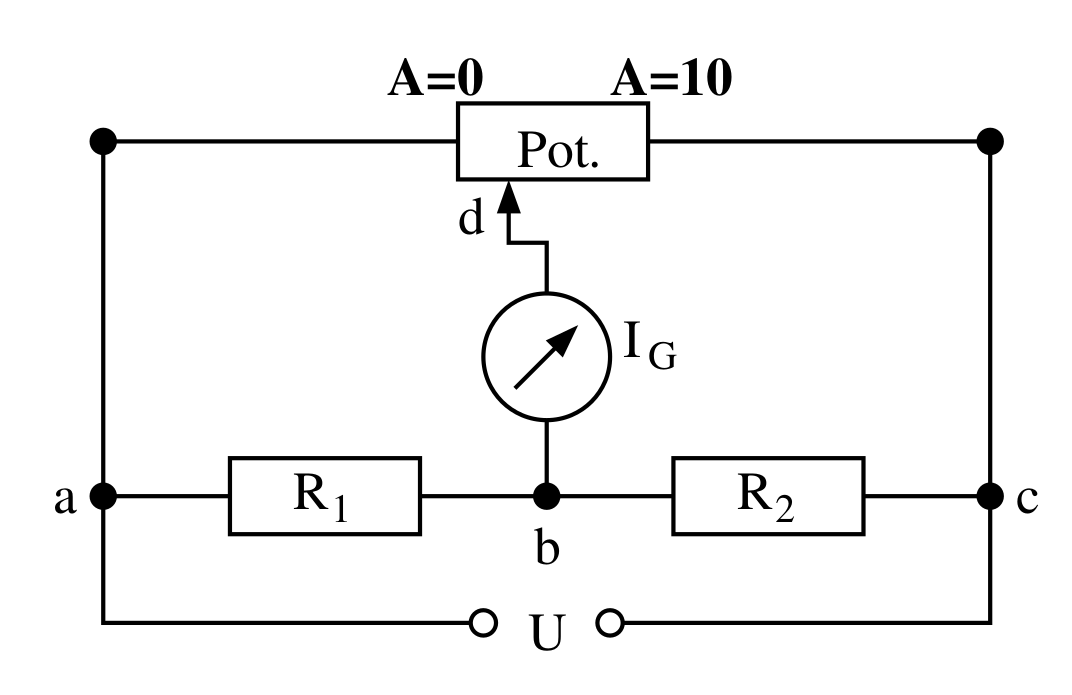
\includegraphics[width=60mm]{graphs/kreis.png}
                \caption{Versuchsaufbau der Wheatstone’schen Brückenschaltung mit Potentiometer}
                \label{fig:kreis}
            \end{figure}
        
            \subsection{Herleitung der Kapazität}
                Man beachte, dass in allen folgenden Kapitel die imaginäre Einheit durch $j$ dargestellt wird, $R_x, I_x$ und $P_x$ den gesuchten Widerstand, Strom und Leistung bezeichnet.
                \\
                Die allgemeine Abgleichbedingung einer Brückenschaltung lautet wie folgt. Diese folgt aus dem Aufbau der Schaltung, falls $I_G = 0$, die Brücke also abgeglichen ist.
                \begin{equation}
                    \owncount
                    \frac{Z_2}{Z_1} = \frac{Z_4}{Z_3}
                    \label{eq:abgleich}
                \end{equation}
                \\
                Dabei lauten die komplexen Widerstände der Schaltung 3 \cite{anleitung}: $\frac{1}{Z_{1}}=\frac{1}{R_{1}}+j \omega C_{1}$, $Z_{2}=R_{2}-\frac{j}{\omega C_{2}}$, $Z_{3}=R_{3}$ sowie $Z_{4}=R_{4}$, mit $\omega$ als Kreisfrequenz.
                Einsetzen in die Abgleichbedingung \ref{eq:abgleich} liefert
                \begin{equation}
                    \owncount
                    \begin{aligned}
                        \left(R_2 - \frac{j}{\omega C_2}\right) \cdot \left(\frac{1}{R1} + j\omega C_x\right) = \frac{R_4}{R_3} \Leftrightarrow \\
                        \frac{C_1}{C_2} + \frac{R_2}{R_1} - j \left(\frac{1}{\omega C_2 R_1} - \frac{C_x \omega}{R_2}\right) = \frac{R_4}{R_3} \quad .
                    \end{aligned}
                \end{equation}
                Da für die rechte Seite Im($\frac{R_3}{R_4}$) = 0, gilt dies auch für die linke Seite.

                \begin{equation}
                    \owncount
                    \frac{1}{\omega C_2 R_1} = \frac{C_x \omega}{R_2} \Rightarrow R_1 = \frac{1}{\omega^2 C_x C_2 R_2}   
                \end{equation}
                Für den Imaginärteil ist $i_g = 0$, die des Realteil wie folgt.
                \begin{equation}
                    \owncount
                    \frac{R_2}{R_2} + \frac{C_x}{C_2} = \frac{R_4}{R_3}
                    \label{eq:abgleich2}
                \end{equation}
                Umstellen der Abgleichbedingung \ref{eq:abgleich2} und einsetzen der Gleichung \ref{eq:wheatstone_abgleich} liefert die Bestimmungsgleichung der unbekannten Kapazität.
                \begin{equation}
                    \owncount
                    C_x = \frac{10-A}{A}\frac{C_2}{R_{2}^{2} \omega^2 C_{2}^{2} +1}
                    \label{eq:bestimmung}
                \end{equation}
    
    
    
    \section{Experimentelles Vorgehen}\label{sec:experiment}
        Bei dem Versuch wurde ein Zehngangpotentiometer mit einem Gesamtwiderstand von \SI{1}{\kilo\ohm} und einer Gesamtlänge der Potentiometerwendel von 10 Umdrehungen verwendet. Die Anzahl der Umdrehungen wird mit A angegeben. In den weiteren Kapiteln folgt eine spezifischere Beschreibung beider Versuchsteile. 
        
        \subsection{Wheatstonesche Brücke}\label{subsec:experiment_wheatstone}
            In diesem Teil wurde der Widerstand von einem unbekannten Widerstand, Spule, Potentiometer und Glühlampe ermittelt.\\
            Bei der ersten Messung sollten die Studenten mit dem Umgang des Potentiometers vertraut gemacht werden. Dafür wurde der Widerstand eines bekannten Widerstandes bei konstanter Spannung U = \SI{1}{\volt} gemessen. Als Vergleichswiderstände $R_v$ benutze man \SI{10}{\ohm}, \SI{30}{\ohm} und \SI{100}{\ohm}.\\
            Beim nächsten Versuch sollte der ohmsche Widerstand bei konstanter Spannung U = \SI{1}{\volt} einer Spule und einer Kupferspule bestimmt werden. Hierfür wurde zuerst der unbekannte Widerstand der Bauteilspule bestimmt. Danach wurde der Widerstand der ganzen Kupferdrahtspule gemessen. Es folgte die Messung an den beiden Abgriffen A\,-\,M und M\,-\,E.\\
            Bei der Messung des ohmschen Widerstandes einer Glühlampe wurde zuerst die Spannung U = \SI{1}{\volt} konstant gehalten. Es wurden die Vergleichswiderstände \SI{10}{\ohm}, \SI{30}{\ohm}, \SI{100}{\ohm} und \SI{200}{\ohm} verwendet.\\
            Danach erfolgte die Messung bei verschiedenen Spannungen von \SI{2}{\volt}, \SI{3}{\volt}, \SI{4}{\volt}, \SI{5}{\volt} und \SI{6}{\volt}. Die verwendeten Vergleichswiderstände waren \SI{10}{\ohm}, \SI{30}{\ohm} und \SI{200}{\ohm}.
            
                
        \subsection{Wechselspannungsbrücke}\label{subsec:experiment_wechsel}
            Für die Messung mit der Wechselspannungsbrücke wurde der Versuchsaufbau umgeändert. Hierbei orientiere man sich passiv an Abbildung 5 der Versuchsanleitung \cite{anleitung}. Es wurde ein Oszilloskop mit eingebautem Funktionsgenerator verwendet. Bei diesem wurde eine Sinusspannung mit einer Frequenz von \SI{1}{\kilo\hertz} und einer maximalen Amplitude von $\leq$ \SI{2}{\volt} eingestellt. Der Oszillator wurde zudem für die Darstellung der Lissajous-Figur verwendet. Diese stellte die Phasenverschiebung von $U_g(t)$ zu $U(t)$ dar. Die dargestellte Lissajous-Figur fand, zusammen mit dem verstellbaren $R_v$, Anwendung in der Abgleichung der Brücke. Um die Brücke abzugleichen, mussten zudem das Potentiometer und $R_v$ so eingestellt werden, dass die Lissajous-Figur eine waagrechte Linie bildete. Hierfür wurden die eingestellten Werte von $A$ notiert. Die Induktivität einer unbekannten Kupferdrahtspule $L_x$ konnte anschließend durch Gleichung \ref{eq:wechsel_abgleich} berechnet werden. Die Berechnung der Kapazität eines unbekannte Kondensators $C_x$ erfolgte durch Gleichung \ref{eq:bestimmung}.
       
            
    
    \section{Ergebnisse}\label{sec:result}
        
        \subsection{Wheatstonesche Brücke}\label{subsec:result_wheatstone}
            Die Messung eines bereits bekannten Widerstands werden in Tabelle \ref{tab:mewh} veranschaulicht. Als Unsicherheit von A wurde 0,05 angenommen. Dieser Wert beinhaltet sowohl die Ablesegenauigkeit, als auch die Unsicherheit des Potentiometers. Die Unsicherheiten der Vergleichswiderstände waren jeweils 1\% ihres angegebenen Widerstandes. Der gewichtete Mittelwert ergab \textbf{(}$\mathbf{104,18 \pm 5,55}$\textbf{)} $\mathbf{\Omega}$. \\ 
            \begin{table}
                \centering
                \begin{tabular}{c|cc}
                    \multicolumn{1}{c}{$R_v$} & \multicolumn{1}{c}{A} & \multicolumn{1}{c}{Ergebnis}\\
                    \cmidrule(l){0-0}\cmidrule(lr){2-2}\cmidrule(lr){3-3}
                    \toprule
                    10 $\Omega$ & 9,15 & $(107,92 \pm 8,03) \Omega$ \\
                    30 $\Omega$ & 7,76 & $(103,93 \pm 4,03) \Omega $ \\
                    100 $\Omega$ & 5,10 & $(104,08 \pm 3,12) \Omega $ \\
                    \bottomrule
                \end{tabular}
                \caption{Messwerte eines bekannten Widerstandes R = 100 $\Omega$ in der Wheatstoneschen Brückenschaltung mit U = 1\si{\volt}.}
                \label{tab:mewh}
            \end{table}
            \\
            Die Messung des ohmschen Widerstandes der Spulen ergab folgenden Ergebnisse.\\
            Die Spule hatte einen Widerstand von \textbf{(}$\mathbf{10,92 \pm 1,31}$\textbf{)}$\,\mathbf{\Omega}$ und die komplette Kupferdrahtspule \textbf{(}$\mathbf{0,65 \pm 0,06}$\textbf{)}$\,\mathbf{\Omega}$. Die beiden Abgriffe ergaben bei A\,-\,M \textbf{(}$\mathbf{0,34 \pm 0,06}$\textbf{)}$\,\mathbf{\Omega}$ und bei M\,-\,E \textbf{(}$\mathbf{0,38 \pm 0,06}$\textbf{)}$\,\mathbf{\Omega}$. Summiert man beide Abgriffe miteinander und errechnet die Unsicherheit kommt man auf einen Gesamtwiderstand von \textbf{(}$\mathbf{0,72 \pm 0,08}$\textbf{)}$\,\mathbf{\Omega}$.\\
            \\
            Bei der letzten Messung wurde anstelle eines unbekannten Widerstandes eine Glühlampe verwendet. Bei einer konstanten Spannung U = \SI{1}{\volt} wurde für $R_v$ \SI{10}{\ohm}, \SI{30}{\ohm}, \SI{100}{\ohm} und \SI{200}{\ohm} verwendet. Es sollten der Widerstand, der Strom und die verbrauchte Leistung der Glühlampe berechnet werden. Ergebnisse sind in Tabelle \ref{tab:gluh} dargestellt\footnote{Der Sourcecode zur Berechnung von $R_x, P_x, I_x$, sowie der Fehler findet sich unter \url{https://github.com/Wegii/AP2-SS19}\label{note:source}}.

            \begin{table}
                \centering
                \begin{tabular}{c|ccc}
                    \multicolumn{1}{c}{} & \multicolumn{3}{c}{Ergebnis} \\
                    \cmidrule(lr){2-4}
                    \toprule
                     $R_v$ [\si{\ohm}]& $R_x$ [$\Omega$]    & $I_x$ [mA]   & $P_x$ [mW] \\ 
                        10  & $46,81 \pm 2,08$      & $20 \pm 3,05$        & $18,72 \pm 7,05$    \\ 
                        30   & $37,72 \pm 1,14$     & $20 \pm 1,97$        & $15,08 \pm 4,75$    \\ 
                        100   & $20,48 \pm 0,93$    & $40 \pm 0,95$        & $32,76 \pm 4,13$    \\ 
                        200   & $12,76 \pm 1,25$    & $70 \pm 0,52$   & $62,52 \pm 8,77 $   \\
                    \bottomrule
                \end{tabular}
                \caption{Errechneter Widerstand, Strom und Leistung unter Betrachtung einer Glühlampe bei U = \SI{1}{V}. Gut erkennbar ist der lineare Zusammenhang zwischen $I$ und $P$.}
                \label{tab:gluh}
            \end{table}

            \begin{figure*}
                \centering
                
                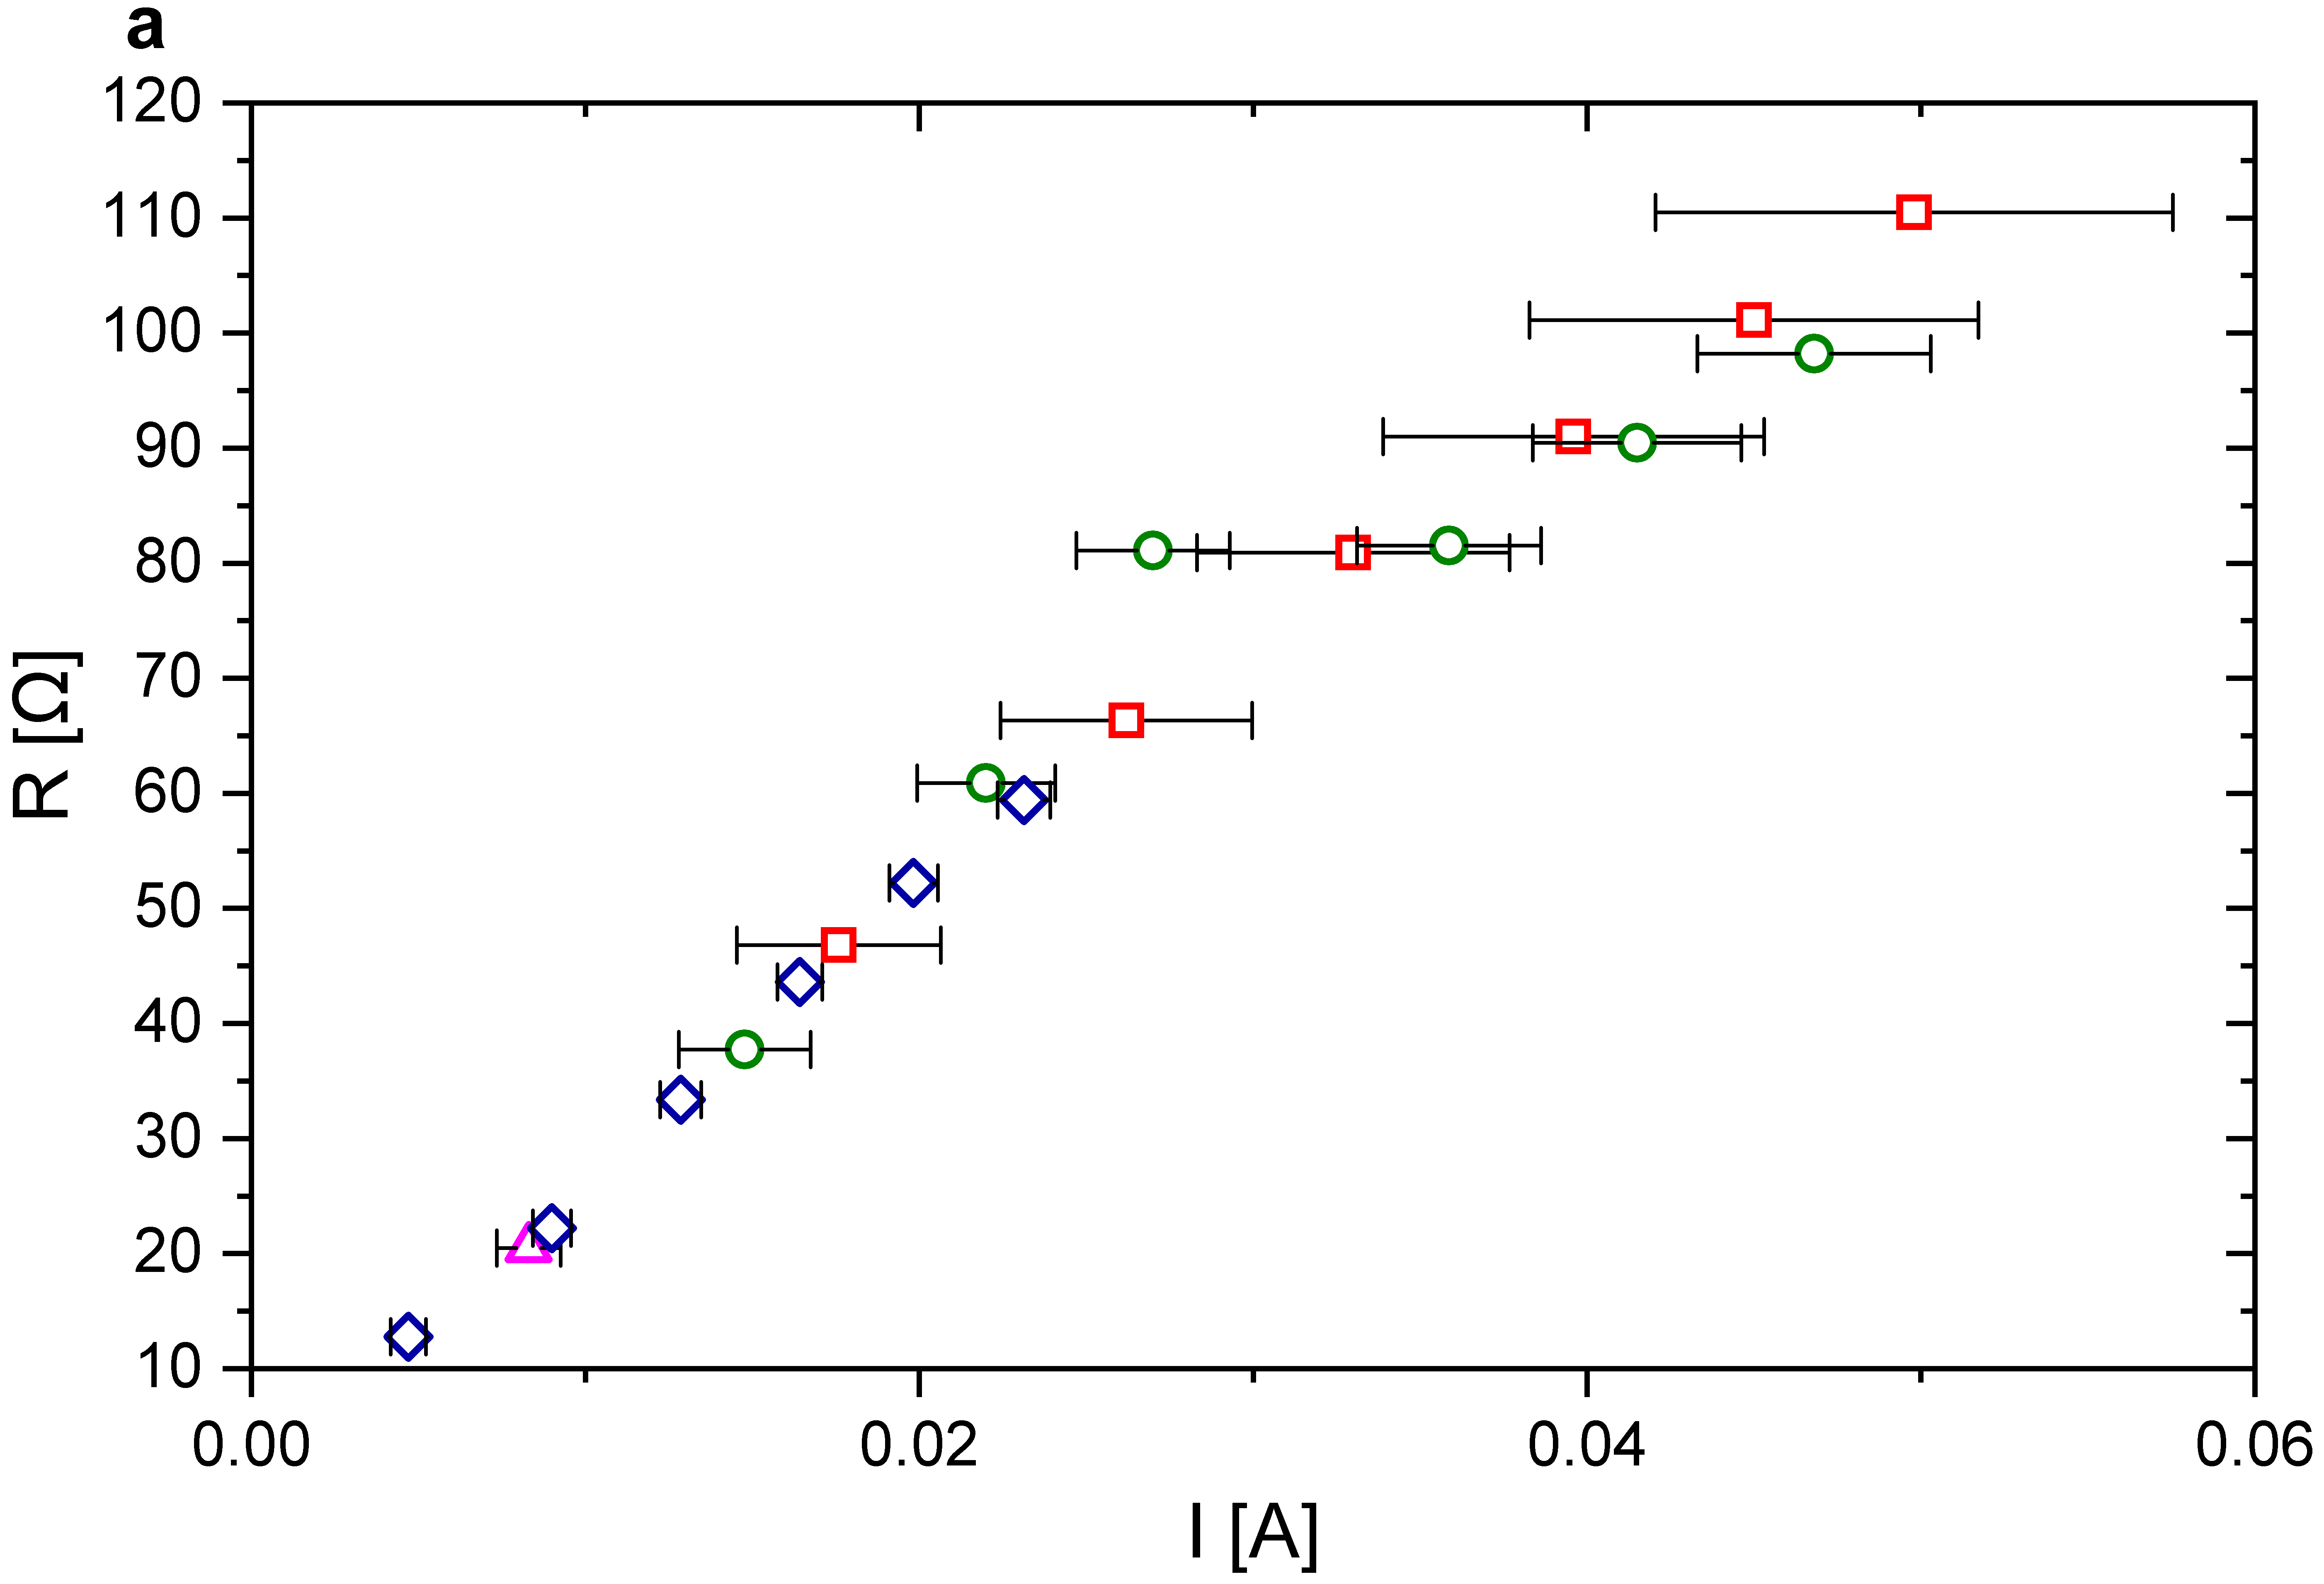
\includegraphics[width=78mm]{graphs/bulbir_res1.png}
                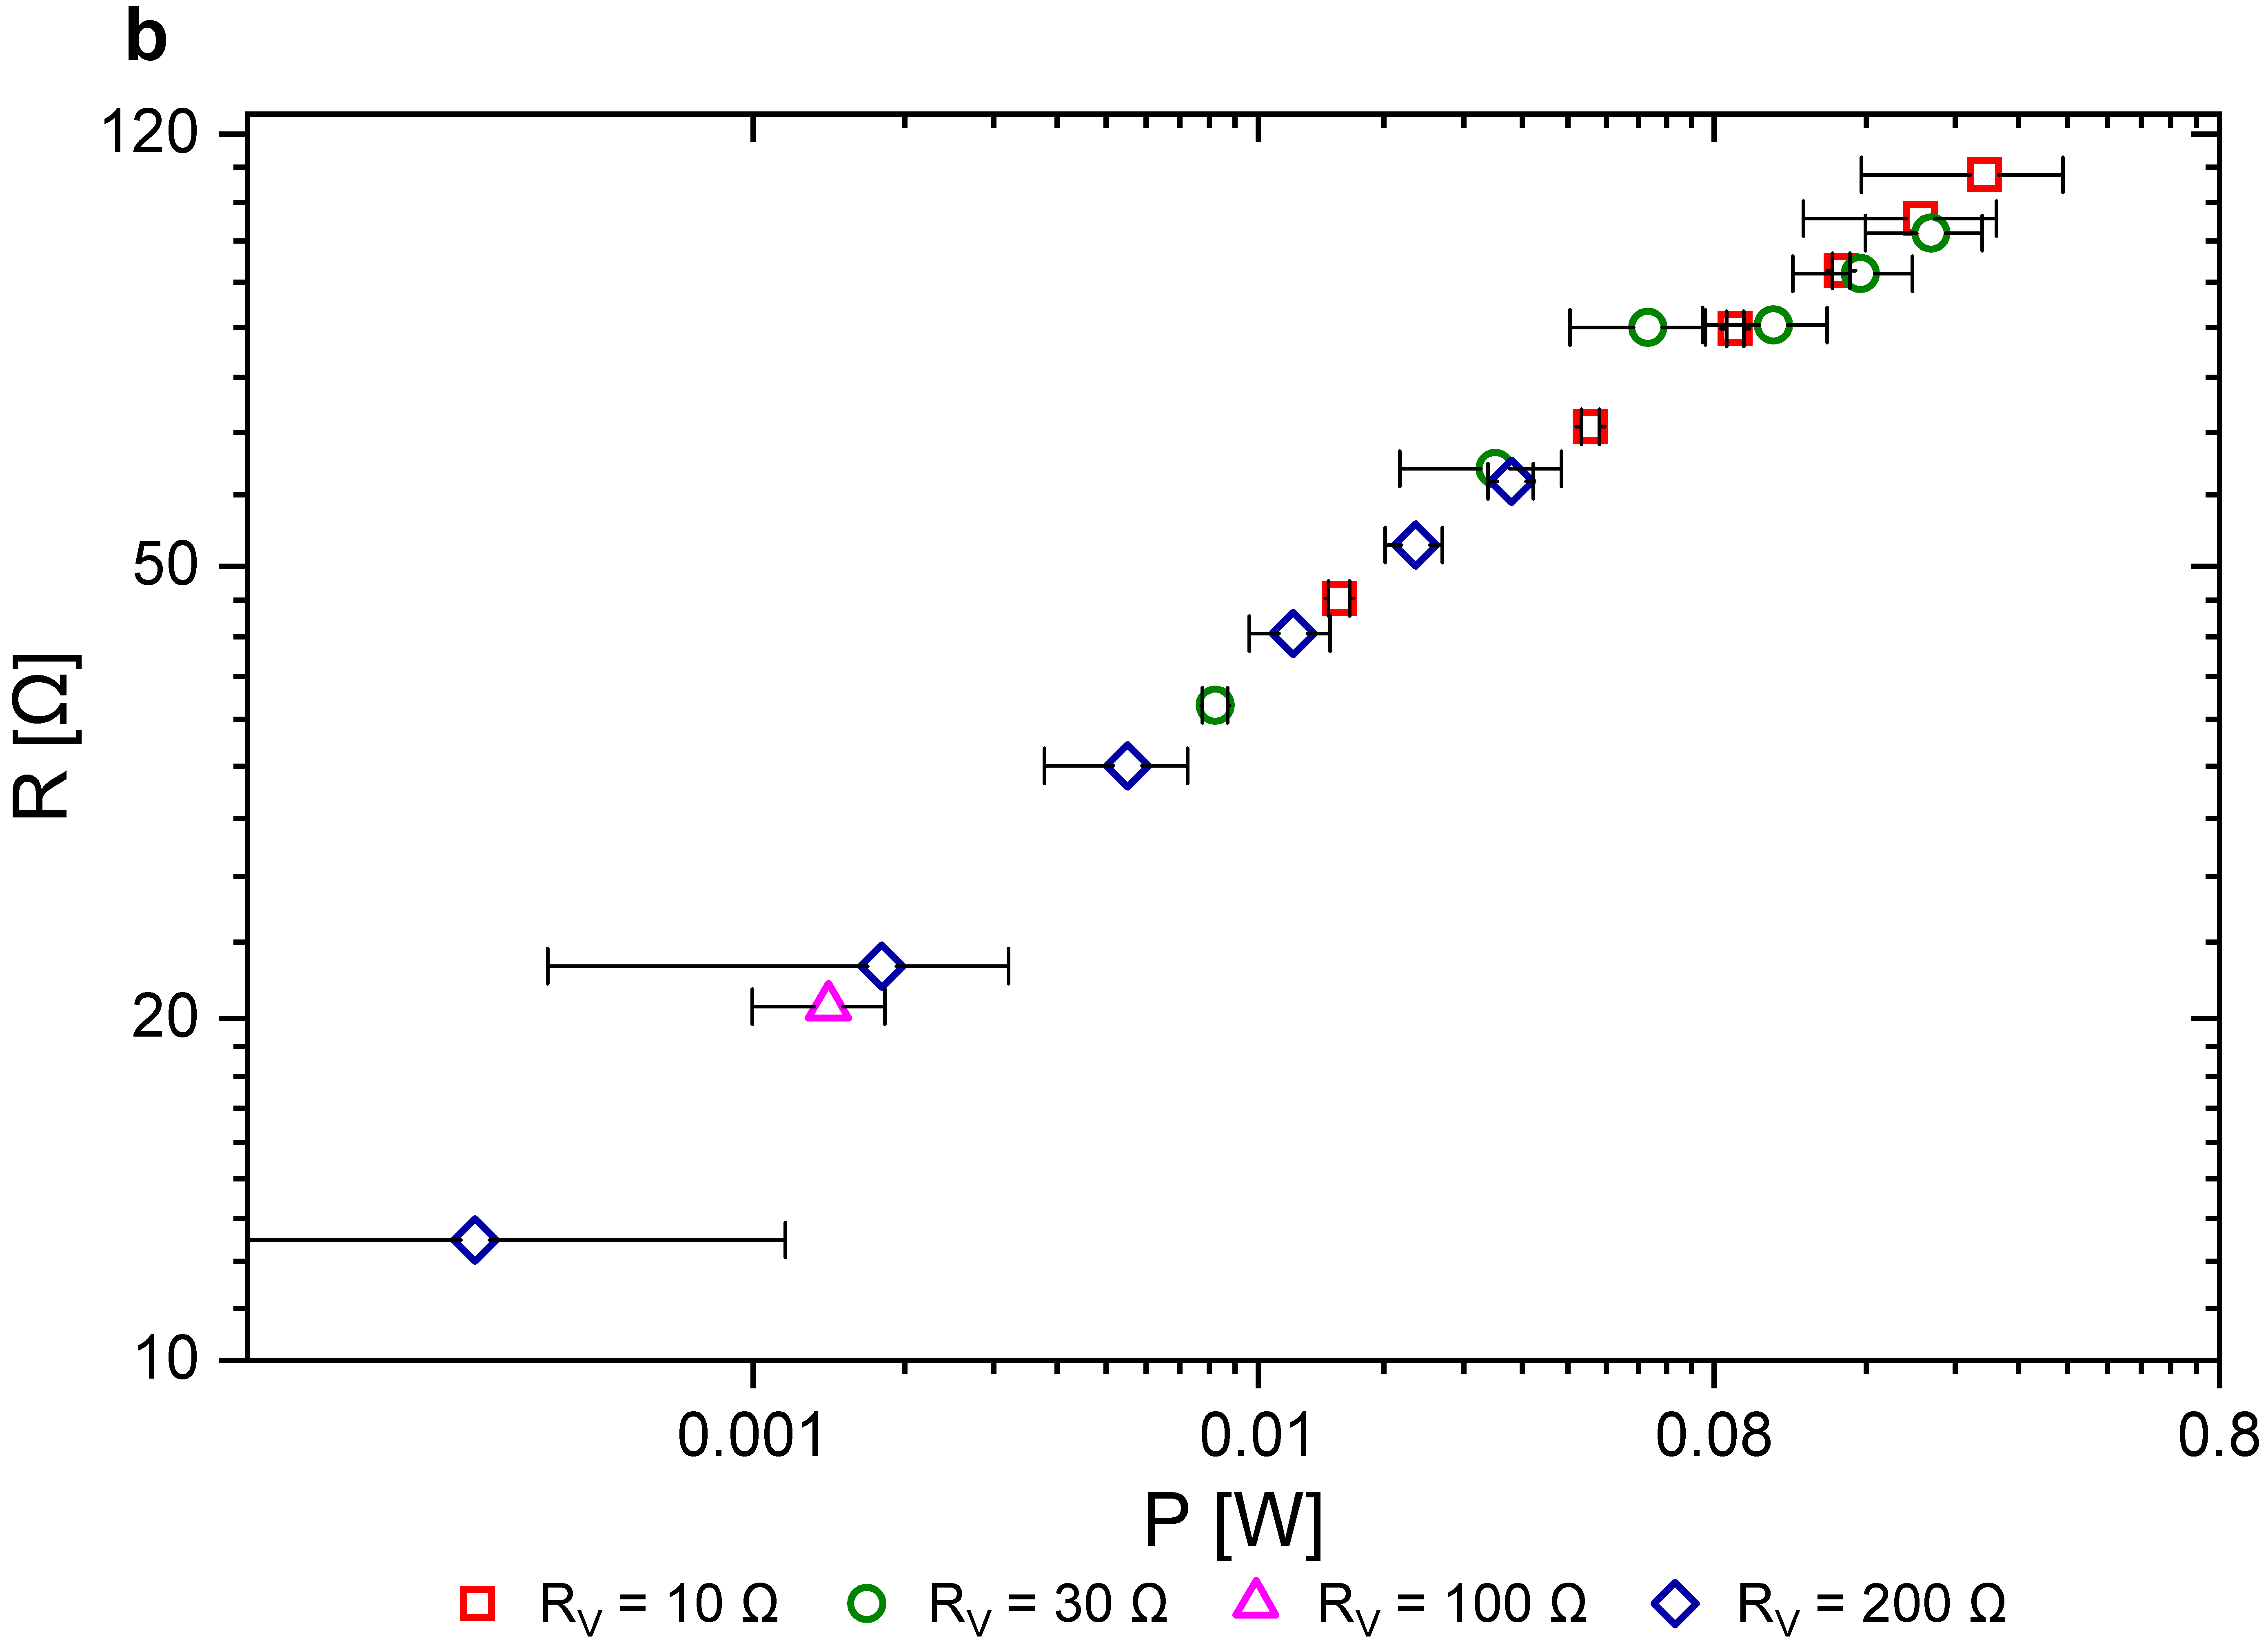
\includegraphics[width=79mm]{graphs/bulbpr_res1.png}
                
                \caption{
                    \textbf{A} I-R-Diagramm in linearer Auftragung. Erkennbarer linearer Anstieg des Widerstands $R_x$ bei Abnahme von $R_v$. Aufgrund des niedrigen resultierenden Widerstands $R_x$, resultiert dies, im Verhältnis zu anderen $R_v$, in einen großen Strom $I$. \\
                    \textbf{B} P-R-Diagramm in doppelt-logarithmischer Auftragung. Linearer Anstieg der Leistung $P$ bei Anstieg von $R_x$. Auch hier resultiert ein kleiner $R_x$ bei der Wahl eines großen $R_v$. Die Wahl eines kleinen $R_v$ führt somit zu einer größeren verbrauchten Leistung $P$ der Glühlampe. 
                    }
                \label{fig:bulb}
            \end{figure*}
            
        
        \subsection{Wechselspannungsbrücke}\label{subsec:result_wechsel}
            Zuerst wurde die Indunktivität der unbekannten Spule ermittelt. Diese beträgt \textbf{(}$\mathbf{1,58 \pm 0,09}$\textbf{)\,mH}. Die Spule wird nun als Vergleichsspule verwendet, um die Induktivitäten der beiden Abgleiche A\,-\,M und M\,-\,E der Kupferspule zu bestimmen. Hierbei ergab sich für A\,-\,M \textbf{(}$\mathbf{0,61 \pm 0,05}$\textbf{)\,mH} und für M\,-\,E \textbf{(}$\mathbf{0,84 \pm 0,07}$\textbf{)\,mH}. Die Unsicherheit der Kupferdrahtspule war mit $(2,7 \pm 0,1)\,$mH gegeben.
            
            \subsubsection{Abgleichbedingung}
                Unter Verwendung der Abgleichbedingung \ref{eq:abgleich} und Bestimmungsgleichung \ref{eq:bestimmung} kann die unbekannte Kapazität $C_x$ berechnet werden. Dabei setzt man $C_v$\,=\,\SI{1}{\micro\farad} und $R_v$\,=\,\SI{42}{\ohm}, wobei $R_v$ abgelesen wurde. Damit ergibt sich ein Wert von
                \begin{center}
                    $\mathbf{C_x = (209,40 \pm 7,00)}$ \textbf{nF} .
                \end{center}

            
    \section{Diskussion}\label{sec:discussion}
        \subsection{Wheatstonesche Brücke}\label{subsec:discussion_wheatstone}
            Bei der Messung des bekannten Widerstandes R\,=\,\SI{100}{\ohm} stimmten die Ergebnisse mit dem gewünschten Wert größtenteils überein. Die Unsicherheit beim Vergleichswiderstand von \SI{100}{\ohm} ist etwas zu klein. Der Grund dafür könnte eine zu klein gewählte Unsicherheit von A sein. Es könnte auch sein, dass die Unsicherheit Von $R_v$\,=\,\SI{100}{\ohm} größer als 1\% ist. Um eine genauere Aussage treffen zu können, hätte man mehr Messungen durchführen müssen. \\
            Sieht man sich jedoch den gewichteten Mittelwert an, befindet sich das Ergebnis um den gewünschten Wert.\\
            \\
            Die beiden Werte bei den halben Abgriffen, A\,-\,M und M\,-\,E,  der Kupferdrahtspule ergeben zusammen etwas mehr als den Gesamtwiderstand der kompletten Kupferdrahtspule. Mit der berücksichtigten Unsicherheit enthält die Summe jedoch den tatsächlichen Widerstand. Die Addidtion der beiden Abgriffe ist gerechtfertigt, da diese sich, theoretisch, in einer Serienschaltung befinden. Ein weitere Grund, weswegen der Widerstand der beiden Abgriffe höher ist, kann der Aufbau der Spule sein. Es muss eine Verbindung zwischen dem mittleren Kontaktpunkt und der halben Spule bestehen. Das heißt, bei der Messung der beiden Abgriffen wird diese Verbindung doppelt gezählt.
            
            
            \subsubsection{Verläufe}
                Im Folgenden werden die zwei Verläufe in Abbildung \ref{fig:bulb} diskutiert. Aufgrund mangelnder Referenzwerte ist es nicht möglich die Ergebnisse der Glühlampe zu vergleichen. Aus Abbildung \ref{fig:bulb}a ist zu erkennen, dass bei zunehmender Spannung, der Widerstand der Glühlampe fast linear zur Stromstärke steigt. Dieser Zusammenhang geht bei dem Vergleichswiderstand von \SI{200}{\ohm} verloren.
                Aus dem Diagramm \ref{fig:bulb}B lässt sich der lineare Zusammenhang zwischen Leistung und Widerstand der Birne ablesen. Je höher die Leistung ist, desto größer wird der Widerstand. Die Steigung ist abhängig vom verwendeten $R_v$. Bei größerem $R_v$ wird die Steigung größer. Bei niedrigem Strom und großen Widerstand $R_x$ verhält sich die Glühlampe wie ein Ohmscher Widerstand und erhält den oben genannten linearen Zusammenhang zwischen Strom und Widerstand. Sobald die Glühlampe anfängt zu glühen, wird der Widerstand durch die zusätzlich Wärmeentwicklung verändert. Bei der Durchführung des Versuchs konnte ein glühen der Glühlampe bei $R_v = 200$ \si{\ohm} festgestellt werden. Aufgrund des kleinen $R_v$ konnte zur Glühlampe mehr Strom fließen, als die Glühwendel abgeben konnte. Infolgedessen erhöht sich die Reibung und Widerstand in der Glühwendel. Der linearer Zusammenhang zwischen Strom und Widerstand ist nicht mehr erhalten. Die bekannte Kennlinie einer Glühlampe, welche einem logarithmischen Zusammenhang folgt, entsteht \cite{tipler}. Dabei erhitzt sich der Draht, bis ein konstante Temperatur angenommen wird. Aufgrund der konvexen Kennlinie handelt es sich bei der Glühlampe um einen Kaltleiter. Selbiges sollte auch in den Kennlinien der anderen $R_v$ sichtbar werden, sobald eine höhere Spannung $U > 6$ angelegt wird. Da für diese $R_v$ grundsätzlich weniger Strom fließt, geschieht dies jedoch langsamer als mit $R_v = 200$ \si{\ohm}. \\
                Bei beiden Verläufen ist auffällig, dass bei dem Vergleichswiderstand $R_v = 30$ \si{\ohm} der Widerstand der Glühlampe bei einer Spannung von $U = 3$ \si{\volt} und $U = 4$ \si{\volt} gleich ist. Es konnte keine physikalische Begründung dafür gefunden werden, und lässt auf einen Ablesefehler schließen.
                
        
        
        \subsection{Wechselspannungsbrücke}\label{subsec:discussion_wechsel}
            Eine Spule erzeugt ein magnetisches Feld. Da in der Schaltung eine Wechselspannung angelegt wurde, erzeugt die somit kontinuierliche Änderung des Magnetfeldes eine weitere Spannung. Da beide Effekte von der Windungszahl proportional abhängen, folgt für die die Induktivität $L_h$ der halben Spule 
            \begin{center}
                $L_h = \frac{L}{4}$ \quad .
            \end{center}
            Dabei ist $L$ die Induktivität der gesamten Spule und kann wie folgt berechnet werden.\\
            \begin{center}
                $L = N^2 \cdot \frac{\mu_0A}{l}$
            \end{center}
            Hierbei ist N die Anzahl der Windungen, l die Länge der Spule, A die Querschnittsfläche der Spule und $\mu_0 = 1,2566 \cdot 10^{-6}$ \si{\frac{N}{A^2}} die magnetische Feldkonstante. 
            Die Induktivität einer halben Spule sollte nur ein viertel der gesamten Spule sein. Auf die im Versuch angewendete Spule bedeutet das also 0,675 \si{\milli\henry}. Diesen Wert wird nur von dem Abgriff M\,-\,E beinhaltet. Der Wert liegt leicht außerhalb des Wertes vom Abgriff A\,-\,M. Die Erklärung ist wieder, dass eine zu kleine Unsicherheit des Potentiometers angenommen wurde, oder der gegebene Wert für die Unsicherheit der Kufperdrahtspule zu klein war. Die Fehlerquelle können auch Rundungsfehler sein. Dieser Fehler würde durch mehrmaliges Messen wahrscheinlich nicht auftreten.\\
            

        
       
    \section{Zusammenfassung}\label{sec:conclusion}
        Es stellte sich heraus, dass mit Hilfe von Brückenschaltungen und der richtigen Einstellung Widerstände, Kapazitäten und Induktivitäten relativ simpel berechnet werden können.\\
        Über die Wheatstonesche Brückenschaltung kann ein unbekannter Widerstand bei dem Vorhandensein von 3 bekannten Widerständen einfach über die Abgleichbedingung \ref{eq:wheatstone_abgleich} bestimmt werden. Dabei ist zu beachten, dass der Spannungsabfall zwischen zwei Punkten innerhalb der Schaltung gleich Null sein muss. Diese Art der Messung ist bei genauer Beachtung der Messungsicherheiten eine gute und einfache Methode um Widerstände zu bestimmen.\\ 
        Bei der Messung mit der Wechselspannungsbrücke können Induktivitäten und Kapazitäten bestimmt werden. Mit Hilfe der Lissajous-Figur, war es möglich die Phasenverschiebung der Spannungen anzugleichen. Damit konnte man über die vereinfachte Gleichung \ref{eq:wechsel_abgleich} die Induktivitäten der Spulen berechnen. Zur Berechnung der Kapazität eines unbekannten Kondensators wurde Gleichung \ref{eq:bestimmung} hergeleitet und verwendet.\\
        Für genauere Messergebnisse und Unsicherheiten hätten die Messversuche öfters wiederholt werden sollen. 
        
    % References
    \bibliographystyle{mnras}
    \bibliography{Ausarbeitung.bib}
    


    % Appendix
    \appendix
    \section{Fehlerrechnung}\label{subsec:fehler}
        Da bei allen Versuchen die Messung nicht wiederholt wurde, handelt es sich bei allen Unsicherheiten von systematischer Natur. Alle Unsicherheiten wurden mittels linearer Addition ermittelt. Die Werte der Unsicherheiten können aus der Tabelle \ref{tab:error} entnommen werden.
        \begin{table}
            \centering
            \begin{tabular}{c|c}
                \multicolumn{0}{c}{Gerät} & \multicolumn{1}{c}{Unsicherheit} \\
                \cmidrule(l){0-0}\cmidrule(lr){2-2}
                \toprule
                    Multimeter $\Delta U$ & 0,1 V      \\ 
                    Kupferdrahtspule  & $(2,1 \pm 0,1)$ mH     \\ 
                    $R_v$  & 1\%       \\ 
                    Potentiometer $\Delta A$  & 0,05      \\
                \bottomrule
            \end{tabular}
            \caption{Systematische Unsicherheiten verwendet in der Fehlerrechnung und den Ergebnissen.}
            \label{tab:error}
        \end{table}
        \\
        Alle genannten Formeln und Methoden sind im Skript zur Fehlerrechnung \cite{fehler} vorzufinden\footnotemark[1]. 
        Für die lineare Addition wurde folgende Formel verwendet.
        \begin{equation}
            \owncount
            \Delta \overline{g} = \left| \Delta \overline{x} \left[\frac{\partial g}{\partial x}\right]_{\overline{x},\overline{y},\overline{z}}\right|\, + \, \cdots
        \end{equation}
        \\
        Um den gewichteten Mittelwertes bei der ersten Messung zu erhalten, wurde zuerst die systematische Unsicherheit jeder Messung berechnet. \\
        Die im Diagramm angegebene Unsicherheiten wurden wie folgt berechnet. 
        \begin{equation}
            \owncount
            \begin{aligned}
                \Delta I = \left|\Delta U \cdot \frac{1}{R_v + R_x}  \right| + \left| \Delta R_v \cdot \frac{-U}{(R_v + R_x)^2}\right|\\
                + \left | \Delta R_x \cdot \frac{-U}{(R_v+ R_x)^2}\right|
            \end{aligned}
        \end{equation}
        \begin{equation}
            \owncount
            \Delta P = |\Delta I\cdot 2 I\cdot R_x| + |\Delta R_x \cdot I^2|
        \end{equation}\\
        Die Unsicherheit des unbekannten Kondensators $C_x$ berechnet sich wie folgt. 
        \begin{equation}
            \owncount
            \begin{aligned}
            \Delta C_x = \left| \Delta A \cdot \frac{C_v}{R_v^2\omega^2C_v^2+1}\frac{-10}{A^2}\right| \\
             + \left| \Delta C_v \cdot \frac{10-A}{A}\frac{1-R_v^2\omega^2C_v^2}{(R_v^2\omega^2C_v^2+1)^2}\right| \\
             + \left| \Delta R_v \cdot \frac{10-A}{A}\frac{-2C_v^3\omega^2R_v}{(C_v^2\omega^2R_v^2+1)^2}\right| 
            \end{aligned}
        \end{equation}


    \label{lastpage}
\end{document}
